%%%%%%%%%%%%%%%%%%%%%%%%%%%%%%%%%%%%%%%%%%%%%%%%%%%%%%%%%%
%%
%%  LOD-L7.tex
%%  Lecture 7: Homotopy Theory in Diffeology
%%
%%%%%%%%%%%%%%%%%%%%%%%%%%%%%%%%%%%%%%%%%%%%%%%%%%%%%%%%%%

\chapter*{\S L7. Homotopy Theory in Diffeology}
\setcounter{footnote}{0}

%%%%%%%%%%%%%%%%%%%%%%%%%%%%%%%%%%%%%%%%%%%%%%%%%%%%%%%%%%
%%
%% MARK: Abstract
%%
%%%%%%%%%%%%%%%%%%%%%%%%%%%%%%%%%%%%%%%%%%%%%%%%%%%%%%%%%%
\begin{abstract}
  This lecture is about homotopy theory in diffeology,
  that generalizes to diffeological spaces the theory of homotopy on Euclidean domains,
  and encompasses the geometric theory of homotopy of manifolds.
  In these times when homotopy can have more than one meaning,
  this theory of homotopy should be understood as the historic version of homotopy,
  built from loops.
  We can specify if necessary and call it the ``geometric homotopy theory of diffeological spaces''.
\end{abstract}

%%%%%%%%%%%%%%%%%%%%%%%%%%%%%%%%%%%%%%%%%%%%%%%%%%%%%%%%%%
%%
%% MARK: Introduction
%%
%%%%%%%%%%%%%%%%%%%%%%%%%%%%%%%%%%%%%%%%%%%%%%%%%%%%%%%%%%

We present the elementary constructions and definitions of the theory of homotopy in diffeology.
In particular,
the definitions of connectedness,
connected components,
homotopic invariants,
the construction of the Poincar\'e groupoid,
the fundamental group and the higher homotopy groups.
We present the relative homotopy,
and the exact sequence of the homotopy of a pair.
Thanks to the functional diffeology on the space of paths of a diffeological space,
we define the higher homotopy groups by considering simply the iteration of its space of loops.
This theory has been originally presented in my doctoral dissertation {\em Fibrations diff\'eologiques et homotopie} \cite{Igl85}.

%%%%%%%%%%%%%%%%%%%%%%%%%%%%%%%%%%%%%%%%%%%%%%%%%%%%%%%%%%
%%
%% MARK:  Smooth Paths and Operations
%%
%%%%%%%%%%%%%%%%%%%%%%%%%%%%%%%%%%%%%%%%%%%%%%%%%%%%%%%%%%
\section{Smooth paths and operations}

\begin{Article}{Smooth paths in a diffeological space.}{}
  We define the set of \emph{smooth paths} in $X$,
  a diffeological space,
  as
  $$%
   \Paths(X) = \Cinfty(\RR,X).
  $$%
  The origin and the end of the path $\gamma$ are defined by
  $$%
  \0(\gamma) = \gamma(0)
  \SpacedText{and}
  \1(\gamma) = \gamma(1).
  $$%
  And the ends of $\gamma$ are naturally defined by
  $$%
  \Ends(\gamma) = (\gamma(0),\gamma(1)).
  $$%
  The set $\Paths(X)$ is equipped with the functional diffeology,
  then:
  $$%
  \0, \1 \in \Cinfty(\Paths(X), X),
  \ \Ends \in \Cinfty(\Paths(X), X \times X).
  $$%
  We generally say ``path'' for ``smooth path'',
  since we almost never consider non-smooth paths.

  \uline{Definition.} {\itshape We say that $x$ and $x'$ are \emph{connected} or \emph{homotopic} if there exists a path such that:
  $$%
  \Ends(\gamma) = (x,x').
  $$%
  }
\end{Article}

\begin{Article}{Smooth loops in a diffeological space.}{}
  A \emph{loop} in $X$ is a path $\gamma$ with same ends,
  that is,
  such that $\0(\gamma) = \1(\gamma)$.
  The space of loops is denoted by $\Loops(X)$,
  $$%
  \Loops(X) = \{ \gamma \in \Paths(X) \mid \0(\gamma) = \1(\gamma) \}.
  $$%
  If we want to specify the \emph{base point},
  $$%
  \Loops(X,x) = \{ \gamma \in \Paths(X) \mid x = \0(\gamma) = \1(\gamma) \}.
  $$%
  Unless otherwise stated,
  all subsets of $\Paths(X)$ are equipped with the subset diffeology.
\end{Article}

\begin{Article}{Concatenating paths.}{}
  \label{Concatenation-Paths}
  Let $X$ be a diffeological space.
  We say that two paths $\gamma$ and $\gamma'$ are \emph{juxtaposable} if
  $$%
  \1(\gamma) = \0(\gamma')
  $$%
  and if there exists a path $\gamma \vee \gamma'$ such that
  $$%
  \gamma\vee\gamma\,'(t) =
  \left\{
  \begin{array}{lcl}
    \gamma(2t) & \mbox{if} & t \leq {1 \over 2}, \\
    \vspace{-5pt} \\
    \gamma'(2t-1) &  \mbox{if} & {1 \over 2} \leq t.
  \end{array}
  \right.
  $$%
  The path $\gamma \vee \gamma'$ is called the \emph{concatenation} of $\gamma$ and $\gamma'$.
\end{Article}

\begin{Article}{Reversing paths.}{}
  \label{Reversing-paths}
  Let $X$ be a diffeological space.
  Let $\gamma$ be a path in $X$, let $x = \0(\gamma)$ and $x' = \1(\gamma)$.
  The path
  $$%
  \bar \gamma \colon t \mapsto \gamma(1-t)
  $$%
  is called the \emph{reverse path} of $\gamma$.
  It satisfies
  $$%
  \0(\bar \gamma) = \1(\gamma)
  \SpacedText{and}
  \1(\bar \gamma) = \0(\gamma).
  $$%
  The map
  $$%
  \Rev \colon \gamma \mapsto \bar \gamma
  $$%
  is  smooth,
  it is an involution of $\Paths(X)$.
  If $\gamma$ and $\gamma'$ are juxtaposable,
  then $\Rev(\gamma')$ and $\Rev(\gamma)$ are juxtaposable,
  and
  $$%
  \Rev(\gamma') \vee \Rev(\gamma) = \Rev(\gamma \vee \gamma').
  $$%
\end{Article} %% Reversing-paths

\begin{Article}{Stationary paths.}{}
  \label{Stationary-paths}
  Let $X$ be a diffeological space.
  We say that a path $\gamma$ is \emph{stationary} at its ends,
  if there exists an open neighborhood of $]-\infty,0]$ and  an open neighborhood of $[+1,+\infty[$ where $\gamma$ is constant.
  Formally,
  the path $\gamma$ is stationary if there exists $\varepsilon > 0$ such that
  %
  $$% %\tag{$\clubsuit$}
    \gamma \restriction \OpenInterval{-\infty, + \varepsilon} = [t \mapsto \gamma(0)]
    \SpacedText{and}
    \gamma \restriction \OpenInterval{1 - \varepsilon, + \infty} = [t \mapsto \gamma(1)].
  $$%
  %
  The set of stationary paths in $X$ is denoted by
  $$%
  \stPaths(X).
  $$%
  The prefix ``st'' is used to denote everything stationary.

  \uline{Note 1.} Two stationary paths $\gamma$ and $\gamma'$ are juxtaposable if and only if $\1(\gamma) = \0(\gamma')$.

  \uline{Note 2.} The concatenation of stationary paths is not associative,
  if $\gamma$, $\gamma'$ and $\gamma''$ are three stationary paths such that
  $$%
  \1(\gamma) = \0(\gamma')
  \SpacedText{and}
  \1(\gamma') = \0(\gamma''),
  $$%
  then $\gamma \vee (\gamma' \vee \gamma'')$ is {\em a priori\/} different from $(\gamma \vee \gamma') \vee \gamma''$.
  For a finite family of stationary paths $(\gamma_k)_{k=1}^n$ such that $\1(\gamma_k) = \0(\gamma_{k+1})$,
  with \hbox{$1\leq k<n$}, %% <- PIZ Adjustment
  we prefer,
  for reasons of symmetry,
  the multiple concatenation defined by
  $$%
  \gamma_1 \vee \gamma_2 \vee \cdots \vee \gamma_n : t
  \mapsto
  \left\{
  \begin{array}{ll}
    \gamma_1(nt - 1 +1) & t \leq {1 \over n}, \\
    \cdots \\
    \gamma_k(nt -k +1 ) & {k -1 \over n} \leq t \leq {k \over n}, \\
    \cdots \\
    \gamma_n(nt-n+1) & {n-1 \over n} \leq t,
  \end{array}
  \right.
  $$%
  which is still a stationary path, connecting $\0(\gamma_1)$ to $\1(\gamma_n)$.
\end{Article} % Stationary-paths

\begin{Article}{Homotopic paths.}{}
    \label{Homotopy-of-paths}
    Let $X$ be a diffeological space.
    Because $\Paths(X)$ is itself a diffeological space,
    it makes sense to say that a path $s \mapsto \gamma_s$ in $\Paths(X)$
    connects $\gamma$ and $\gamma'$, that is,
    $$%
    [s \mapsto \gamma_s] \in \Paths(\Paths(X)) = \Cinfty(\RR, \Paths(X)),
    $$%
    with  $\gamma_0 = \gamma$ and $\gamma_1 = \gamma'$.

    $\bullet$ \emph{Free-ends homotopy.}
    Such a path $\gamma \mapsto \gamma_s$ is called a free-ends homotopy,
    connecting $\gamma$ to $\gamma'$,
    or from $\gamma$ to $\gamma'$.

    $\bullet$ \emph{Fixed-ends homotopy.}
    Now,
    let $\Paths(X,x,x')$ be the set of paths in $X$ connecting $x$ to $x'$,
    equipped with the subset diffeology of $\Paths(X)$.
    A path $[s \mapsto \gamma_s] \in \Paths(\Paths(X,x,x')) =  \Cinfty(\RR,\Paths(X,x,x'))$ is called a \emph{fixed-ends homotopy} from $\gamma$ to $\gamma'$.
    But note that,
    by definition of the subset diffeology,
    $[s \mapsto \gamma_s]$ is a fixed-ends homotopy if and only if $[s \mapsto \gamma_s] \in \Paths(\Paths(X))$ and for all $s \in \RR$, $\gamma_s(0) = x$ and $\gamma_s(1) = x'$.

    \smuline{Proposition.} {\itshape A crucial property of homotopy in diffeology is that every path $\gamma$ is fixed-ends homotopic to a stationary path.}

    Indeed,
    let us consider the \emph{smashing function\/} $\lambda$ described in Figure \ref{fig-smashing-function},
    where $\varepsilon$ is some strictly positive real number, $0 < \varepsilon \ll 1$.
    The real function $\lambda$ satisfies essentially the following conditions, and we can choose it increasing,
    $$%
    \lambda \in \Cinfty(\RR,\RR), \ \lambda \restriction \OpenInterval{-\infty,\varepsilon} = 0, \ \lambda \restriction \OpenInterval{1-\varepsilon, + \infty} = 1.
    $$%
    Let $\gamma \in \Paths(X)$.
    We have the following properties:
    \enlargethispage{1mm} %%% <- PIZ Adjustment
    %
    \begin{itemize}
      \item[a)] The path $\gamma^\star = \gamma \circ \lambda$ is stationary with the same ends as $\gamma$.
      \item[b)] The path $\gamma$ is fixed-ends homotopic to $\gamma^\star$.
    \end{itemize}
    
    \begin{figure}[t!]
      \centerline{
\includegraphics[width=.33\textwidth]{Figures/fig-smashing-function}}
      \caption{The smashing function $\lambda$.}
      \label{fig-smashing-function}
    \end{figure}

   \uline{Note.} As we know, not any two paths $\gamma, \gamma' \in \Paths(X)$ such that $\1(\gamma) = \0(\gamma')$ can be juxtaposable,
   but we can always force the concatenation by smashing them first.
   Hereafter,
   we shall often use this \emph{smashed concatenation},
   denoted and defined by
    $$%
    \gamma \star \gamma' = \gamma^\star \vee \gamma'^\star.
    $$%
    As a consequence of the point b),

    \smuline{Proposition.} {\itshape If $\1(\gamma) = \0(\gamma')$,
    then $\gamma \star \gamma'$ connects $\0(\gamma)$ to $\1(\gamma')$.
    Moreover,
    if $\gamma$ and $\gamma'$ are juxtaposable,
    then $\gamma \vee \gamma'$ is homotopic to $\gamma \star \gamma'$.
    }
\end{Article} % Homotopy-of-paths

\begin{Article}{Connected components.}{}
  Let $X$ be a diffeological space.

  \uline{Proposition 1.} {\itshape To be connected,
  or homotopic,
  is an equivalence relation on $X$ whose classes are called \emph{connected components}.
  The connected component of $x \in X$ is denoted by
  $$%
  \Comp(x) = \{ x' \in X \mid \exists \gamma \in \Paths(X), \Ends(\gamma) = (x,x') \}.
  $$%
  The set of components is denoted by
  $$%
   \pi_0(X) = \{ \Comp(x) \mid x \in X \}.
  $$%
  Equipped with the quotient diffeology,
  $\pi_0(X)$ is discrete.
  }

  Let $x \in X$,
  we denote by $\pi_0(X,x)$ the pointed space:
  $$%
   \pi_0(X,x) = (\pi_0(X), x).
  $$%

  \uline{Proposition 2.} {\itshape If $X$ is connected,
  then
  $$%
  \Ends \colon \Paths(X) \to X \times X
  $$%
  is a subduction.}
\end{Article}

\begin{Article}{The sum of its components.}{}
  \label{The-sum-of-its-components}
  Let $X$ be a diffeological space.
  The space $X$ is the sum of its connected components.
  More precisely,
  if $X$ is the sum of a family $\{X_i\}_{i \in \cI}$,
  then the connected components of the $X_i$ are the connected components of $X$.
  The decomposition of $X$ into the sum of its connected components is the finest decomposition of $X$ into a sum.
  It follows that the set of components $\pi_0(X)$,
  equipped with the quotient diffeology of $X$ by the relation \emph{connectedness},
  is discrete.
\end{Article} %% The-sum-of-its-components

\begin{Article}{Higher homotopy groups.}{}
  \label{Higher-homotopy-groups}
  Let $X$ be a diffeological space,
  and let $x$ be a point in $X$.
  The \emph{higher homotopy groups} of $X$,
  based at $x$,
  are defined recursively.
  Let us denote by $\hat x$ the constant loop
  $$%
   \hat x \colon t \mapsto x.
  $$%
  Then,
  we define,
  for all integer $n > 0$:
  $$%
  \pi_n(X,x) = \pi_{n-1}(\Loops(X,x), \hat x),
  $$%

  For $n=1$ it gives
  $$%
  \pi_1(X,x) = \pi_0(\Loops(X,x), \hat x) = (\pi_0(\Loops(X,x)), \hat x),
  $$%
  which is called the \emph{fundamental group} of $X$, based at $x$.

  \smuline{Proposition.} {\itshape The set $\pi_1(X,x)$ is equipped with a multiplication defined by:
  $$%
   \Class(\ell) \cdot \Class(\ell') = \Class(\ell \vee \ell'),
  $$%
  for all $\ell,\ell' \in \Loops(X,x)$.
  This multiplication gives $\pi_1(X,x)$ a group structure:
  \begin{itemize}
  \item[a)] the identity is $\Class(\hat x)$,
  \item[b)] the inverse of $\Class(\ell)$ is $\Class(\bar \ell)$,
  where $\bar \ell$ is the reverse of $\ell$.
  \end{itemize}
  }

  \smuline{Proposition.} {\itshape If $x$ and $x'$ are connected,
  then the groups $\pi_1(X,x)$ and $\pi_1(X,x')$ are conjugate.}

  Now, let us define the recurrence
  \begin{eqnarray*}
  \Loops_{n+1}(X,x) & = & \Loops(\Loops_n(X,x), \hat x_n), \\
  \SpacedText{and}
  \hat x_{n+1} & = & [t \mapsto \hat x_n],
  \end{eqnarray*}
  initialized by
  $$%
  \Loops_0(X,x) = X
  \SpacedText{and}
  \hat x_0 = x.
  $$%
  We have then:
  $$%
  \pi_n(X,x) = \pi_0(\Loops_n(X,x), \hat x_n),
  $$%
  for all $n \in \NN$.
  For $n \geq 1$,
  $\pi_n(X,x) = \pi_1(\Loops_{n-1}(X,x), \hat x_{n-1})$,
  which shows that the higher homotopy groups of $X$ are the fundamental groups of some loop spaces,
  and therefore deserve their name of ``group''.

  \uline{Note 1.} This is specific to diffeology since in traditional differential geometry the set of loops of a manifold is not a manifold,
  and talking about the $\pi_1$ of a set of loops has no well-founded meaning.

  For example,
  $\pi_2(X,x)$ is the fundamental group of the connected component of the constant loop $\hat x$ in $\Loops(X,x)$ etc.
  Since loop spaces are H-spaces,
  the groups $\pi_n(X,x)$ are Abelian for $n \geq 2$.

  \uline{Note 2.} Let $f \colon X \to X'$ be a smooth map,
  then $f$ induced a map from $\pi_n(X,x)$ to $\pi_n(X',x')$,
  with $x' = f(x)$,
  which is a group morphism for all $n > 0$ and a morphism of pointed space for $n = 0$.
\end{Article}

\begin{Article}{The Poincar\'e groupoid and fundamental group.}{}
  \label{The-Poincare-groupoid-and-fundamental-group}
  Let $X$ be a diffeological space.
  Let $\Pi$ be the equivalence relation on $\Paths(X)$\,:
  $$%
    \gamma \mathop{\Pi} \gamma' \ \Leftrightarrow \
    \left\{\begin{array}{l}
      \mbox{there exists } x,x' \in X \mbox{ and } \xi \in \Paths(\Paths(X,x,x')) \\
      \vspace{-10pt} \\
      \mbox{such that } \xi(0) = \gamma \mbox{ and } \xi(1) = \gamma'.
    \end{array}
    \right.
  $$%
  Said differently,
  $\gamma$ and $\gamma'$ belong to the same component of
  $$%
  \Paths(X,x,x'),
  $$%
  the subspace of paths such that $\Ends(\gamma) = \Ends(\gamma') = (x,x')$.
  We shall denote by $\Pi(X)$ the
  diffeological quotient $\Paths(X)/\Pi$,
  and by $\Class$ the canonical projection:
  $$%
  \Class \colon \Paths(X) \to \Pi(X) = \Paths(X)/\Pi.
  $$%
  We shall denote again by $\Ends$ the factorization of $\Ends \colon \Paths(X) \to X \times X$ on $\Pi(X)$.

  Note that, if $X$ is connected, then $\Ends : \Pi(X) \to X \times X$ is a subduction,
  and $\Class \restriction \stPaths(X) \to \Pi(X)$ is also a subduction.

  The \emph{Poincar{\'e} groupoid} $\Poinc{X}$ is then defined by
  $$%
  \Obj(\Poinc{X}) = X
  \SpacedText{and}
  \Mor(\Poinc{X}) = \Pi(X).
  $$%
  For all $x$ and $x'$ in $X$,
  $$%
  \Mor_{\Poinc{X}}(x,x') = \Paths(X,x,x')/\Pi = \pi_0(\Paths(X,x,x'))
  $$%
  is \uline{the set of fixed-ends homotopy classes of the paths connecting $x$ to $x'$}.
  The composition in the groupoid is the projection of the concatenation of paths.
  For all $\tau \in \Mor_{\Poinc{X}}(x,x')$ and $\tau' \in \Mor_{\Poinc{X}}(x',x'')$,
  $$%
  \tau \cdot \tau' = \Class(\gamma \vee \gamma'),
  \SpacedText{where}
  \tau = \Class(\gamma)
  \SpacedText{and}
  \tau' = \Class(\gamma').
  $$%
  The paths $\gamma$ and $\gamma'$ are chosen in $\stPaths(X)$, for the
  concatenation $\gamma \vee \gamma'$ to be well defined.

  The construction of the Poincar{\'e} groupoid is
  summarized by the following diagram.
  \begin{center}
    \begin{tikzpicture}[auto]
      \node (A)  at (-2.5,0) {$\Paths(X)$};
      \node (B)  at (2.5,0) {$\Pi(X)$};
      \node (C)  at (0,-2.2) {$X \times X$};
      \draw[->] (A) to node {$\Class$} (B);
      \draw[->] (A) to node [swap] {$\Ends$} (C);
      \draw[->] (B) to node {$\Ends$} (C);
    \end{tikzpicture}
  \end{center}
  The isotropy groups ${\Poinc{X}}_x = \Mor_{\Poinc{X}}(x,x)$ and the inverse of the elements of ${\Poinc{X}}(x,x') = \Mor_{\Poinc{X}}(x,x')$ are described by what follows:
  \begin{itemize}
    \item[a)] For every point $x$ of $X$,
    the isotropy group $\Id_x \in {\Poinc{X}}_x$ is the component $\Class(\hat x)$,
    in $\Loops(X,x)$,
    of the constant path $\hat x$.
    \item[b)] The inverse $\tau^{-1}$ of $\tau = \Class(\gamma) \in \Mor_{\Poinc{X}}(x,x')$ is the component $\Class(\bar \gamma)$ of the reverse path $\bar \gamma = \Rev(\gamma)$.
  \end{itemize}
  The structure group ${\Poinc{X}}_x = \Mor_{\Poinc{X}}(x,x)$,
  where $x \in X$,
  is the first homotopy group,
  or the fundamental group,
  of $X$ at the point $x$.
  That is,
  $\pi_1(X,x)$.

  If $X$ is connected,
  then the fundamental groups
  are isomorphic.
  They are precisely conjugate,
  if $\tau \in \Mor_{\Poinc{X}}(x,x')$,
  then
  $$%
  \pi_1(X,x) = \tau \cdot \pi_1(X,x') \cdot \tau^{-1}.
  $$%
  In this case,
  the type of the homotopy groups $\pi_1(X,x)$ is denoted by $\pi_1(X)$.

  \uline{Definition.} {\itshape The space $X$ is said to be {\em simply connected} if it is connected,
  $\pi_0(X) = \{X\}$,
  and if its fundamental group $\pi_1(X)$ is trivial.
  In that case $\Ends \colon \Pi(X) \to X \times X$ is a diffeomorphism.}

  \uline{Note.} If $X$ is not connected, then $\pi_1(X,x)$ is also the fundamental group of the connected component of $x$,
  that is,
  $\pi_1(X,x) = \pi_1(\Comp(x),x) = \pi_1(\Comp(x))$,
  since there is one type of fundamental group by component.
\end{Article} %% The-Poincare-groupoid-and-fundamental-group

\begin{Article}{The universal covering.}{}
  Let $X$ be a connected diffeological space,
  let $\Pi(X)= \Paths(X)/\Pi$ the space of morphisms of the Poincaré groupoid.

  \smuline{Proposition.} {\itshape The preimage
  $$%
  \tilde X_x = \Ends^{-1}(\{x\} \times X)
  $$%
  is a simply connected diffeological space.
  The projection
  $$%
  \pi = \1 \restriction \tilde X_x
  $$%
  is a principal fiber bundle with group $\pi_1(X,x)$.
  The spaces $\tilde X_x$ and $\tilde X_{x'}$ are equivalent and denoted generally by $\tilde X$.
  }

  The space $\tilde X$ is called the \emph{universal covering} of $X$.
\end{Article}

\begin{Article}{Monodromy Theorem.}{}
  Let $\pi \colon \tilde X \to X$ be the universal covering of a connected diffeological space.
  Let $f \colon Y \to X$ be a smooth map,
  where $Y$ is simply connected.

  \uline{Theorem.} {\itshape There exists a smooth global lifting $\tilde f \colon Y \to \tilde X$.
  Let $y \in Y$,
  $x = f(y)$ and $\tilde x \in \pi^{-1}(x)$,
  then there is a unique lifting $\tilde f$ such that $\tilde f(y) = \tilde x$.
  }
\end{Article}

\begin{proof}
Let $y' \in Y$ and $t \mapsto y_t$ a smooth path such that $y_0 = y$ and $y_1 = y'$.
Let $x_t = f(y_t)$,
$t \mapsto x_t$ is a path pointed at $x = f(y)$.
Let
$$%
 \tilde f(y') = \Class[t \mapsto x_t].
$$%
This is a lift of $f$.
And $\tilde f(y')$ does not depend on the special choice of the path $t \mapsto y_t$ because $Y$ is simply connected.
\end{proof}

%%%%%%%%%%%%%%%%%%%%%%%%%%%%%%%%%%%%%%%%%%%%%%%%%%%%%%%%%%
%%
%% MARK:  Every Topological Space Admits a Universal Covering
%%
%%%%%%%%%%%%%%%%%%%%%%%%%%%%%%%%%%%%%%%%%%%%%%%%%%%%%%%%%%
\section{Every topological space admits a universal covering}

For the topologist this sentence ``Every topological space admits a universal covering'' is incorrect,
because every topologist is aware of the theorem:

\uline{Topology theorem}~{\itshape A pathwise connected topological space admits a simply connected covering if and only if it is semi-locally simply connected.}

However,
as an application of the theory of diffeology homotopy and the previous construction of the Poincaré groupoid and subsequent universal covering,
we get the following theorem,
which is also true:

\begin{Article}{The universal covering of a topological space.}{}
  Consider a pathwise connected topological space $X$,
  equip $X$ with the \emph{topo-diffeology} for which the plots are the continuous parametrizations.
  This diffeology was introduced at first by Paul Donato in his thesis \cite{Don84}.

  Thus,
  as a diffeological space,
  $X$ admits a simply connected diffeological covering $\pi \colon \tilde X \to X$,
  for which the projection $\pi$ is continuous.

  Indeed,
  the continuous paths,
  which are parametrizations by definition,
  are smooth for the topo-diffeology.
  Then,
  $X$ equipped with the topo-diffeology is connected and the construction (\textsection\,\ref{The-Poincare-groupoid-and-fundamental-group}) applies.

  Therefore,
  every topological space admits a universal covering,
  in the sense of diffeology.

  We have to note that the D-topology of the topo-diffeology is {\em a priori} finer than the initial topology.
  It contains {\em a priori} more open sets.
  Moreover,
  we shall see later that every diffeological space is locally path-connected,
  for the D-topology.

  Note also that in diffeology the projection $\pi \colon \tilde X \to X$ is not {\em a priori} a local diffeomorphism,
  nor a local homeomorphism.

  There are here many conjectures we can investigate about the relationship between this universal covering and the pure topological situation.

  Diffeology gives us a procedure to smooth the space,
  even if it is not semi-locally simply connected,
  which is enough to give it a unique universal covering.

  Let us recall that in topology a covering is a map $\pi \colon \tilde X \to X$ which is locally equivalent,
  in the sense of topology,
  to a direct product with a discrete fiber.
\end{Article}

%%%%%%%%%%%%%%%%%%%%%%%%%%%%%%%%%%%%%%%%%%%%%%%%%%%%%%%%%%
%%
%% MARK:  Relative Homotopy
%%
%%%%%%%%%%%%%%%%%%%%%%%%%%%%%%%%%%%%%%%%%%%%%%%%%%%%%%%%%%
\section{Relative homotopy}

  We describe now the homotopy of a pair $(X,A)$,
  where $X$ is a diffeological space and $A$ is a subspace of $X$.
  We establish the short and long exact sequences of the homotopy of the pair $(X,A)$,
  pointed at $a \in A$,
  which is a key ingredient of the exact homotopy sequence of the diffeological fiber bundles.

\begin{Article}{The short homotopy sequence of a pair.}{}
  \label{The-short-homotopy-sequence-of-a-pair}
  Let $X$ be a diffeological space,
  let $A$ be a subspace of $X$,
  and let $a \in A$.
  Let
  $$%
  \Paths(X,A,a) = \{ \gamma \in \Paths(X) \mid \0(\gamma) \in A \text{ and } \1(\gamma) = a \}.
  $$%
  Let $\gamma$ and $\gamma'$ be two paths belonging to $\Paths(X,A,a)$,
  a \emph{homotopy from $\gamma$ to $\gamma'$,
  relative to $A$,
  pointed at $a$} is a path in $\Paths(X,A,a)$,
  connecting $\gamma$ to $\gamma'$.
  We shall also call it an $(A,a)$-relative homotopy from $\gamma$ to $\gamma'$.
  In Figure \ref{fig-relativeHomotopyOfAPair} the paths $\gamma$ and $\gamma'$ belong to $\Paths(X,A,a)$,
  with $A = A_1 \cup A_2$.
  The path $\gamma$ is $(A,a)$-relatively homotopic to a loop in $X$,
  but not $\gamma'$.
  %%###########
  \begin{figure}[htb]
    \centerline{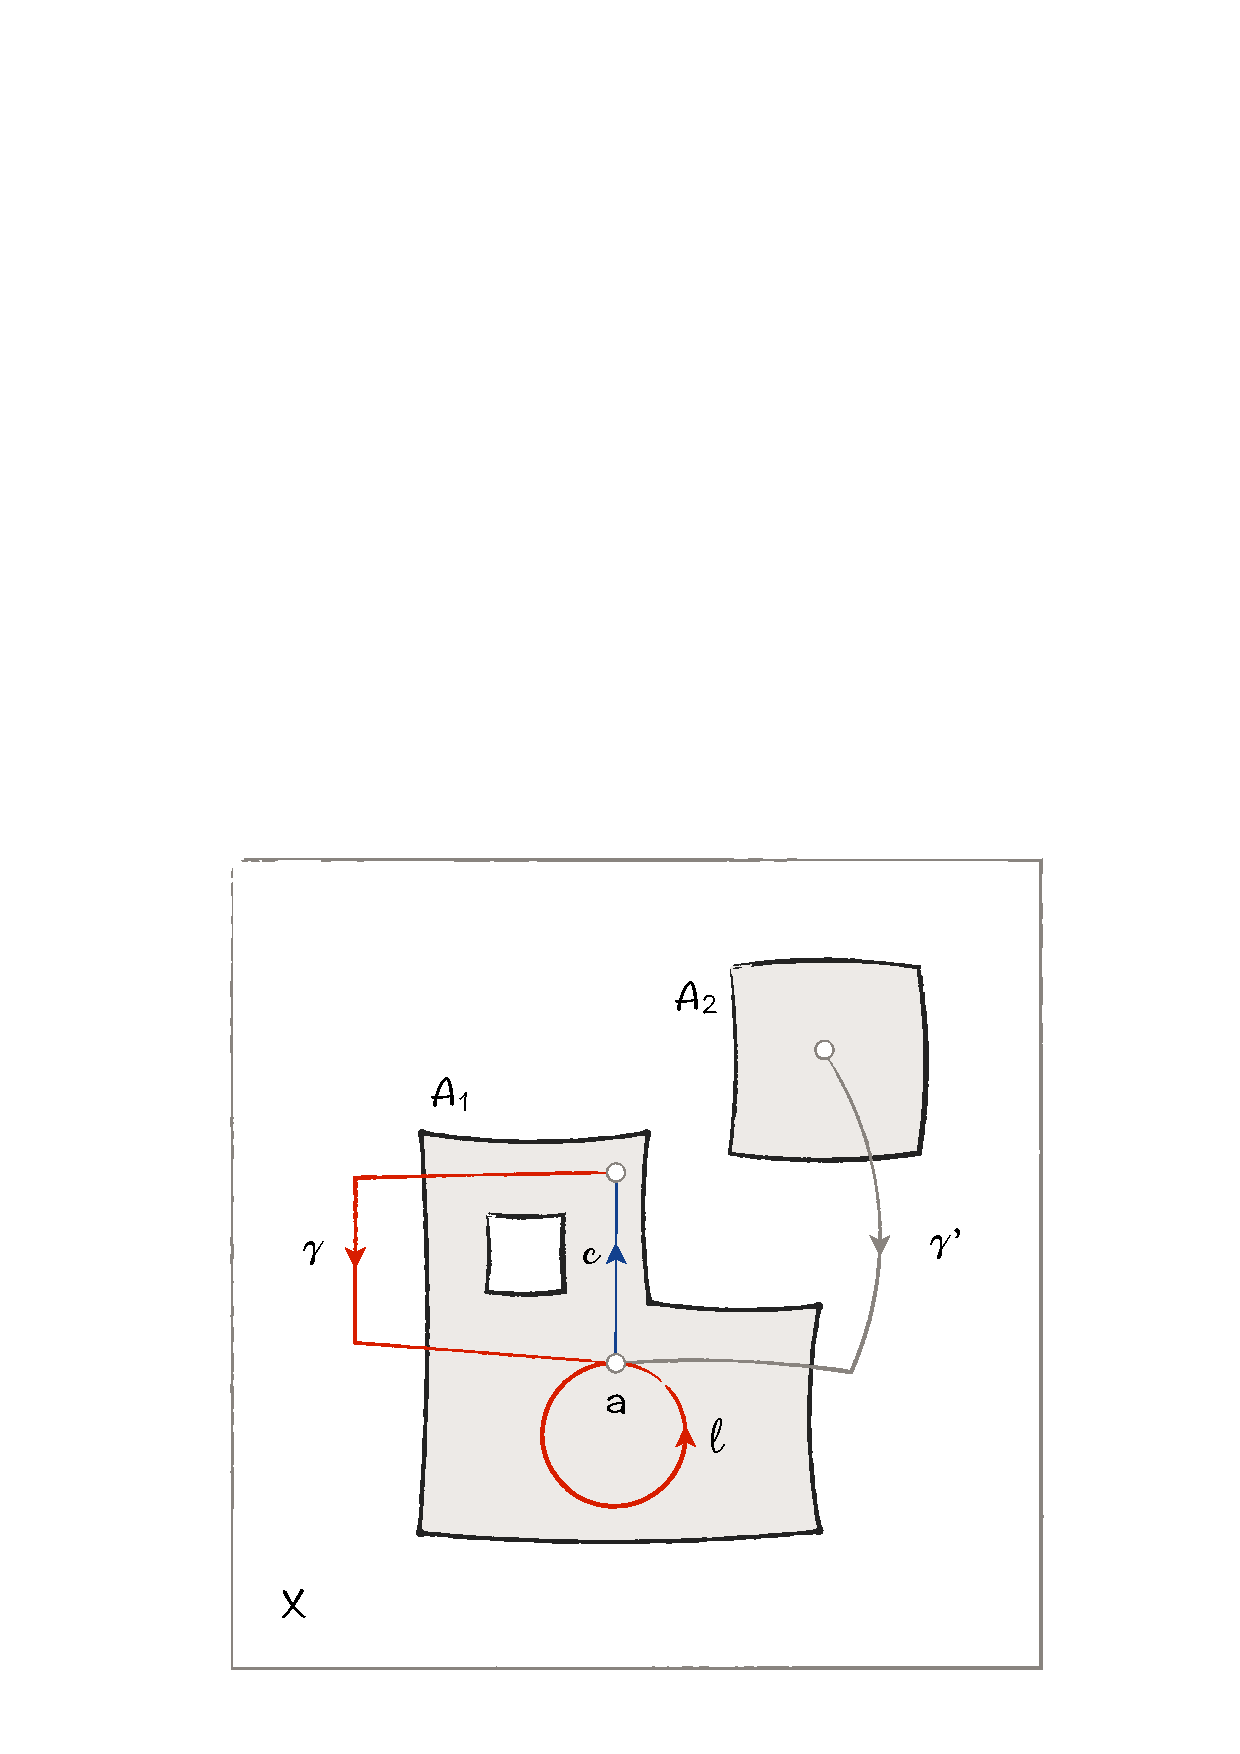
\includegraphics[width=0.55\textwidth]{Figures/relative-homotopy.pdf}}
    \caption{Relative homotopy of a pair.}
    \label{fig-relativeHomotopyOfAPair}
  \end{figure}
  %%###########
  Let us consider the map
  $$%
  \0 \colon \Paths(X,A,a) \to A
  $$%
  and the injection
  $$%
  i \colon A \to X.
  $$%
  They form a two-terms sequence of smooth maps:
  $$%
  \Paths(X,A,a) \rfl{\0} A \rfl{i} X.
  $$%
  This sequence induces naturally the two-terms sequence of morphisms of pointed spaces,
  $$%
  (\Paths(X,A,a),\hat a) \rfl{\0} (A,a) \rfl{i} (X,a),
  $$%
  where $\hat a = [t \mapsto a]$.
  Then,
  this sequence induces a two-terms sequence on the space of components
  \begin{equation}
    \renewcommand{\theequation}{$\heartsuit$}
    \pi_0(\Paths(X,A,a),\hat a) \rfl{\0_\#} \pi_0(A,a) \rfl{i_\#} \pi_0(X,a).
  \end{equation}

  \uline{Note 1.} $\ker(i_\#)$ --- The {\em
  kernel} of $i_\#$ is the subset of components of $A$,
  contained in the component of $X$ containing $a$.

  \uline{Note 2.} $\Val(\0_\#)$ --- The {\em values} of $\0_\#$ are the components of $A$,
  containing the initial points of the paths in $X$ starting in $A$ and ending at $a$.
  In other words,
  the subset of the components of $A$ which can be connected,
  through $X$,
  to $a$.
  Now,
  it is clear that any component of $A$ which can be connected to $a$ by a path in $X$ is included in the component of $X$ containing $a$.
  Conversely,
  every component of $A$ included in the component of $X$ containing $a$ can be connected to $a$ by a path in $X$,
  starting in $A$. So, we get the equality,
  $$%
  \ker(i_\#) = \Val(\0_\#).
  $$%
  Now,
  let us consider the inclusion of the triple $(X,a,a)$ into $(X,A,a)$.
  It induces an injection,
  denoted by $j$,
  on the space of paths,
  $$%
  \Paths(X,a,a) = \Loops(X,a) \rfl{j} \Paths(X,A,a).
  $$%
  This injection descends,
  on the space of components,
  into a morphism of pointed spaces,
  \begin{equation}
    \renewcommand{\theequation}{$\diamondsuit$}
    \pi_0(\Loops(X,a),\hat a) \rfl{j_\#} \pi_0(\Paths(X,A,a), \hat a).
  \end{equation}
  Now,
  the concatenation of $(\diamondsuit)$ to the two-terms sequence $(\heartsuit)$ gives a three-terms sequence of morphisms of pointed spaces,
  \begin{equation} \renewcommand{\theequation}{$\spadesuit$}
    \begin{array}{c}
    \pi_0(\Loops(X,a),\hat a)  \rfl{j_\#}  \pi_0(\Paths(X,A,a),\hat a))  \rfl{\0_\#} \\
    \pi_0(A,a)  \rfl{i_\#} \pi_0(X,a).
    \end{array}
  \end{equation}
  Let us call,
  by abuse of language,
  {\em first group of homotopy of $X$,
  relative to $A$,
  pointed at $a$},
  the pointed space denoted by $\pi_1(X,A,a)$,
  and defined by
  $$%
  \pi_1(X,A,a) = \pi_0(\Paths(X,A,a), \hat a).
  $$%
  Since,
  by definition,
  $\pi_0(\Loops(X,a),\hat a) = \pi_1(X,a)$
  ---~regarded as pointed space~---
  the sequence of morphisms $(\spadesuit)$ rewrites,
  \begin{equation}
    \renewcommand{\theequation}{$\clubsuit$}
    \pi_1(X,a) \rfl{j_\#}
    \pi_1(X,A,a) \rfl{\0_\#}
    \pi_0(A,a) \rfl{i_\#} \pi_0(X,a).
  \end{equation}
  This sequence is called the {\em short sequence of the relative homotopy of the pair $(X,A)$,
  at the point $a$}.
  We have seen that
  $$%
  \ker(i_\#) = \Val(\0_\#);
  $$%
  moreover,
  $$%
  \ker(\0_\#) = \Val(j_\#).
  $$%

  \uline{Note 3.} $\ker(\0_\#)$ --- The kernel of $\0_\#$ is the set of the components of $\Paths(X,A,a)$ whose initial point belongs to the component of $A$ containing $a$.

  \uline{Note 4.} $\Val(j_\#)$ --- The values of $j_\#$ are the components of the $\gamma \in \Paths(X,A,a)$  which are $(A,a)$-relatively homotopic to some loops in $X$, based at $a$.

  In short,
  the relative homotopy sequence of the pair $(X,A)$,
  at the point $a$, is exact.
\end{Article} %% The-short-homotopy-sequence-of-a-pair

\begin{proof}
  We need only check that
  $$%
  \ker(\0_\#) = \Val(j_\#).
  $$%
  Let us recall that,
  on the one hand,
  $\ker(\0_\#)$ is made up of the components of $\Paths(X,A,a)$ whose initial point belongs to the same component of $A$,
  containing $a$.
  On the other hand, $\Val(j_\#)$ is the set of the components of paths $\gamma \in \Paths(X,A,a)$ which are $(A,a)$-relatively homotopic to some loops in $X$,
  based at $a$.

  \uline{Note 1.} $\Val(j_\#) \subset \ker(\0_\#)$.
  If a path $\gamma$ is $(A,a)$-relatively homotopic to some loop in $X$ based at $a$,
  its initial point is connected,
  in $A$,
  to $a$,
  and belongs to the same component of $A$ containing $a$.

  \uline{Note 2.} $\ker(\0_\#) \subset \Val(j_\#)$.
  Let us consider a component of $A$ contained in the same component of $X$ containing $a$.
  Let $\gamma$ be a stationary path in $X$,
  beginning in $A$ and ending at $a$ such that its beginning belongs to the component of $A$ containing $a$.
  Let $\gamma(0) = x$.
  Since $x$ and $a$ belong to the same component of $A$,
  there exists a stationary path $c$ in $A$ connecting $a$ to $x$ (Figure \ref{fig-relativeHomotopyOfAPair}).
  Let $\xi(s) = [t \mapsto c(s + (1-s)\lambda(t))]$,
  where $\lambda$ is the smashing function.
  Thus,
  $\xi$ belongs to $\Paths(\Paths(X,A,a))$ and $\xi(s)(1) = c(1) = x = \gamma(0)$.
  So,
  $\sigma(s) = \xi(s) \vee \gamma$ is a homotopy connecting $(c \circ \lambda) \vee \gamma \in \Loops(X,a)$ to $\hat x \vee \gamma$,
  which is homotopic to $\gamma$.
  Therefore $\gamma$ is $(A,a)$-relatively homotopic to a loop in $X$,
  based at $a$.
\end{proof}

\begin{Article}{The long homotopy sequence of a pair.}{}
  \label{The-long-homotopy-sequence-of-a-pair}
  Let $X$ be a diffeological space,
  let $A$ be a subspace of $X$,
  and let $a \in A$.
  Let us denote again by $i$ the natural induction $i \colon \Loops(A,a) \to  \Loops(X,a)$.
  There is no ambiguity with the injection $i$ of \textsection\,\ref{The-short-homotopy-sequence-of-a-pair},
  since the spaces involved are not the same.
  Then,
  let us consider the two-terms sequence of smooth maps
  $$%
  \Paths(\Loops(X,a),\Loops(A,a), \hat a) \rfl{\0} \Loops(A,a) \rfl{i} \Loops(X,a).
  $$%
  Or,
  if we prefer,
  by denoting
  $$%
  X_1 = \Loops(X,a), \quad A_1 = \Loops(A,a) \SpacedText{and} a_1 = [t \mapsto a],
  $$%
  the above two-terms sequence of smooth maps writes
  $$%
  \Paths(X_1,A_1, a_1) \rfl{\0} A_1 \rfl{i} X_1.
  $$%
  We can then apply the construction of the previous paragraph and get the short sequence of relative homotopy of the pair $(X_1,A_1)$,
  at the point $a_1$.
  Let us denote again by $j$ the natural induction from $\Loops(X_1,a_1)$ to $\Paths(X_1,A_1,a_1)$.
  Thus,
  we have,
  \begin{equation}
    \renewcommand{\theequation}{$\diamondsuit$}
    \pi_1(X_1,a_1) \rfl{j_\#}
    \pi_1(X_1,A_1,a) \rfl{\0_\#}
    \pi_0(A_1,a_1) \rfl{i_\#} \pi_0(X_1,a_1).
  \end{equation}
  Let us define the second group of relative homotopy of the
  pair $(X,A)$,
  at the point $a$,
  by
  $$%
  \pi_2(X,A,a) =
  \pi_1(X_1,A_1,a_1) =
  \pi_0(\Paths(X_1,A_1,a_1),a_1).
  $$%
  So,
  the short exact sequence $(\diamondsuit)$ writes now
  \begin{equation}
    \renewcommand{\theequation}{$\heartsuit$}
    \pi_2(X,a) \rfl{j_\#}
    \pi_2(X,A,a) \rfl{\0_\#}
    \pi_1(A,a) \rfl{i_\#} \pi_1(X,a).
  \end{equation}
  But the right term $\pi_1(X,a) \!=\! \pi_0(X_1,a_1)$ is just $\pi_0(\Loops(X,a),\hat a)$,
  that is,
  $\pi_1(X,a)$,
  regarded as a pointed space.
  It is also the left term of the relative homotopy sequence of the pair $(X,A)$ at the point $a$.
  Let us connect the right term of the short homotopy sequences relative to the pair $(X_1,A_1)$,
  to the left term of the short homotopy sequences relative to the pair $(X,A)$.
  We get
  \begin{multline*}
  \cdots
  \pi_2(X,A,a) \rfl{\0_\#}
  \pi_1(A,a) \rfl{i_\#}
  \pi_1(X,a) \rfl{j_\#} \\
  \pi_1(X,A,a) \rfl{\0_\#}
  \pi_0(A,a) \cdots
  \end{multline*}
  Then,
  let us describe the connection of the morphisms of these two relative homotopy sequences at the junction $\pi_1(X,a)$.

  \uline{Note 1.} $\ker(j_\# : \pi_1(X,a) \to \pi_1(X,A,a))$ --- This kernel is the set of classes of loops of $X$ based at $a$ which can be connected,
  relatively to $(A,a)$,
  to the constant loop $\hat a$.

  \uline{Note 2.} $\Val(i_\# : \pi_1(A,a) \to \pi_1(X,a))$ --- This is the set of classes of loops in $X$,
  based at $a$,
  that are fixed-ends homotopic to a loop in $A$.

  Now, if a loop in $X$,
  based at $a$,
  can be smoothly deformed into a loop contained in $A$,
  then it can be retracted relatively to $A$ into the constant loop $\hat a$.
  Conversely,
  if a loop of $X$,
  based at $a$,
  is connected relatively to $(A,a)$ to the constant loop $\hat a$,
  then it is fixed-ends homotopic to a loop in $A$.
  In other words,
  $$%
  \ker(j_\# \colon \pi_1(X,a) \to \pi_1(X,A,a)) = \Val(i_\# : \pi_1(A,a) \to \pi_1(X,a)).
  $$%
  Thus, the connection of the two short exact relative homotopy sequences is exact.
  Now, let us define the \emph{higher relative homotopy groups} of the pair $(X,A)$ at the point $a$ by recursion.
  Let us remark first that the inclusion $i \colon A \to X$ induces an inclusion
  $$%
  i_n : \Loops_n(A,a) \to \Loops_n(X,a).
  $$%
  Then,
  we can define
  $$%
  \Paths_{n+1}(X,A,a) = \Paths(\Loops_n(X,a),\Loops_n(A,a), \hat a_n),
  $$%
  for every integer $n$,
  and this gives the higher relative homotopy groups
  \begin{eqnarray*}
    \pi_{n+1}(X,A,a) &  = & \pi_0(\Paths_{n+1}(X,A,a),\hat a_n) \\
    & = & \pi_1(\Loops_n(X,a),\Loops_n(A,a), \hat a_n).
  \end{eqnarray*}
  Now,
  we can iterate the above connection of short relative homotopy sequences for each degree $n+1 \to n$,
  and we get \emph{the long exact relative homotopy sequence of the pair $(X,A)$, at the point $a$}.
  \begin{equation*}
    %\renewcommand{\theequation}{$\clubsuit$}
    \left.
    \begin{array}{r@{\hspace{-2pt}}c@{\hspace{-2pt}}c@{\hspace{-2pt}}c@{\hspace{-2pt}}c@{\hspace{-2pt}}c@{\hspace{-2pt}}c@{\hspace{0pt}}l@{\hspace{-2pt}}l}
      \cdots \rfl{i_\#} &  \pi_n(X,a) & \rfl{j_\#} & \pi_n(X,A,a) & \rfl{\0_\#} & \pi_{n-1}(A,a) & \rfl{i_\#} & \pi_{n-1}(X,a) \cdots\,
      \\
      \vspace{-5pt}
      \\
      \cdots \rfl{i_\#} &  \pi_1(X,a) & \rfl{j_\#} & \pi_1(X,A,a) & \rfl{\0_\#} & \pi_0(A,a)     & \rfl{i_\#} & \pi_0(X,a).
    \end{array}
    \right\}
  \end{equation*}
\end{Article} %% The-long-homotopy-sequence-of-a-pair

\begin{proof}
  We need only check that
  $$%
  \ker(j_\# : \pi_1(X,a) \to \pi_1(X,A,a))
  $$%
  is equal to
  $$%
  \Val(i_\# : \pi_1(A,a) \to \pi_1(X,a)).
  $$%
  Let us recall that $\ker(j_\#)$ is made up of the loops of $X$ based at $a$ which can be connected,
  relatively to $(A,a)$,
  to the constant loop $\hat a$,
  and $\Val(i_\#)$ is the subset of the classes of loops in $X$,
  based at $a$,
  which are fixed-ends homotopic to a loop in $A$.

  \uline{Note 1.} $\ker(j_\#) \subset \Val(i_\#)$.
  Let $\ell$ be a loop in $X$,
  based at $a$,
  $(A,a)$-relatively homotopic to the constant loop $\hat a$.
  Let $\gamma$ be the homotopy.
  So,
  for all $s \in \RR$,
  $$%
  \gamma(0) = \ell, \quad \gamma(1) = \hat a, \quad
  \gamma(s)(0) \in A \SpacedText{and} \gamma(s)(1) = a.
  $$%
  The properties of $\gamma$ are schematized in Figure
  \ref{fig-relativeHomotopyOfLoop}.
  %%###########
  \begin{figure}[htb]
    \centerline{\includegraphics[width=.55\textwidth]{Figures/relative-homotopy-II.pdf}}
    \caption{A relative homotopy of a loop to the constant loop.}
    \label{fig-relativeHomotopyOfLoop}
  \end{figure}
  %%###########
  Let us consider a line of $\RR^2$,
  turning around the origin,
  its intersection with the cube describes a homotopy connecting $\ell$ to $\gamma_{t=0} \in \Loops(A,a)$.
  More precisely, let us consider first the path $\gamma' : s \mapsto [t \mapsto \gamma(t)(st)]$  in $\Loops(X,a)$.
  The path $\gamma'$ connects $\ell$ to $[t \mapsto \gamma(t)(t)]$.
  Then,
  let us consider the path $\gamma'' : s \mapsto [t \mapsto \gamma((1-s)t)(t)]$ in $\Loops(X,a)$.
  The path $\gamma''$ connects $[t \mapsto \gamma(t)(t)]$ to $\gamma_{s=0} \in \Loops(A,a)$.
  Therefore,
  $\ell$ is $(A,a)$-relatively homotopic to a loop in $A$, based at $a$.

  \uline{Note 2.} $\Val(i_\#) \subset \ker(j_\#)$. Let $\Comp(\gamma) \in \Val(i_\#)$.
  We can choose $\gamma \in \Loops(A,a)$.
  The path $\xi : s \mapsto [t \mapsto \gamma(s + (1-s)t)]$ is a $(A,a)$-relative homotopy connecting $\gamma$ to the constant loop $\hat a$.
\end{proof}

\begin{Article}{The long homotopy sequence of a fiber bundle.}{}
  Consider a diffeological fiber bundle $\pi \colon Y \to X$ with fiber $F$,
  then the long exact sequence of a pair induces a long exact sequence of the fiber bundle
  \begin{equation*}
    %\renewcommand{\theequation}{$\clubsuit$}
    \left.
    \begin{array}{r@{\hspace{-2pt}}c@{\hspace{-2pt}}c@{\hspace{-2pt}}c@{\hspace{-2pt}}c@{\hspace{-2pt}}c@{\hspace{-2pt}}c@{\hspace{0pt}}l@{\hspace{-2pt}}l}
      \cdots \rfl{i_\#} &  \pi_n(Y,y) & \rfl{\pi_\#} & \pi_n(X,x) & \rfl{\partial} & \pi_{n-1}(F,y) & \rfl{i_\#} & \pi_{n-1}(Y,y) \cdots\,
      \\
      \vspace{-5pt}
      \\
      \cdots \rfl{j_\#} & \pi_1(X,x) & \rfl{\partial} & \pi_0(F,y)     & \rfl{i_\#} & \pi_0(Y,y) & \rfl{\pi_\#} & \pi_0(X,x).
    \end{array}
    \right\}
  \end{equation*}

\end{Article} %% The-long-homotopy-sequence-of-a-fiber-bundle

\vfill
\centerline{\includegraphics[width=1\textwidth]{Figures/Notes-Homotopy.pdf}}
